%% Présentation du sujet du stage [2-4 pages]
\label{sujet}
J'ai intégré l'équipe \textit{Carte acoustique} pendant mon stage d'ingénieur.\\

Le stage proposé s’inscrit dans le cadre de l’optimisation d’un système d’authentification forte dont le mot de passe dynamique est généré en acoustique.\\

Le format du système d’authentification sera préférentiellement celui d’une carte bancaire mais pourra également revêtir celui d’une mini calculette. L'un des objectifs du stage est de fiabiliser la signature acoustique: celle-ci devra prendre en compte les requis des systèmes de télécommunications, les contraintes des formats proposés et les spécifications électroniques. Les informations inclues dans le message acoustique devront pouvoir être déconvoluées puis traitées avec un pourcentage de succès important, celui-ci sera notamment déterminé en fonction de conditions opératoires variables.\\

\section{Plate-forme de tests}

Maintenant la carte est en version 4G (V4G: quatrième génération de smartcard), qui est fonctionnelle et attend les tests. Les tests ont pour  objectif d'évaluer la performance de carte en différents aspects, par exemple:\\

\begin{itemize}
\item Taux de récupération avec différents périphériques et conditions
\item Fiabilité de l'encryptage
\item Durée de vie
\item etc...\\
\end{itemize}

C'est le stagiaire qui est le responsable de concevoir le plan de test et de l'implémenter.
\newpage
\section{Plate-forme de démonstration}

Maintenant UINT possède une plate-forme de démonstration, un site pour montrer l'utilisation de la carte acoustique figuré ci-dessous, mais les fonctionnalités sont très limites. Un nouveau site de démonstration, plus complet et abondant est nécessaire.

\begin{figure}[!htbp]
  \centering
    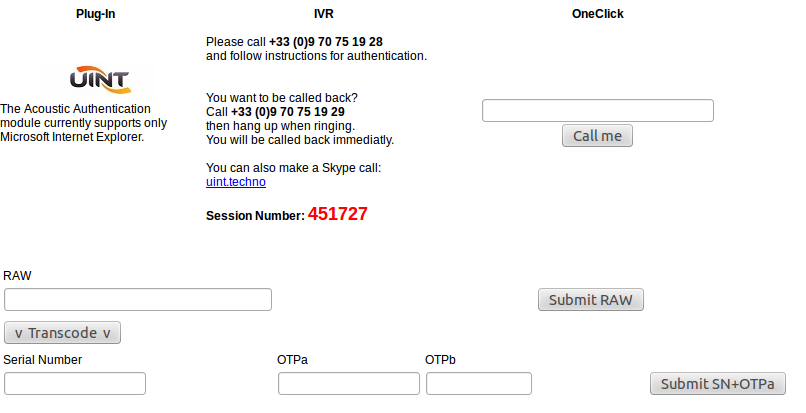
\includegraphics[scale=0.5]{images/d6}
    \caption{Site de démonstration \texttt{acoustictechno}}
\end{figure}


Le nouveau site (par exemple un site d'achat en ligne) doit contenir au moins les fonctionnalités suivantes:\\

\begin{itemize}
\item Utiliser la carte acoustique comme un moyen d'authentification par un utilisateur déjà inscrit
\item Utiliser la carte acoustique comme un moyen de paiement avec les différents possibilités 
  \begin{itemize}
  \item avec navigateur Web
  \item avec téléphone ou mobile
  \end{itemize}
\item Autres à définir
\end{itemize}


















